%!TEX root = main.tex

\section{Important Note} % (fold)
\label{sec:important_note}
\begin{itemize}
	\item Do not use this product outside the country of purchase as it may violate the wireless telecommunication and power regulations of that country.
\end{itemize}
% section important_note (end)
\section{Device Overview} % (fold)
\label{sec:device_overview}
\begin{figure}[tbh!]
	\centering
	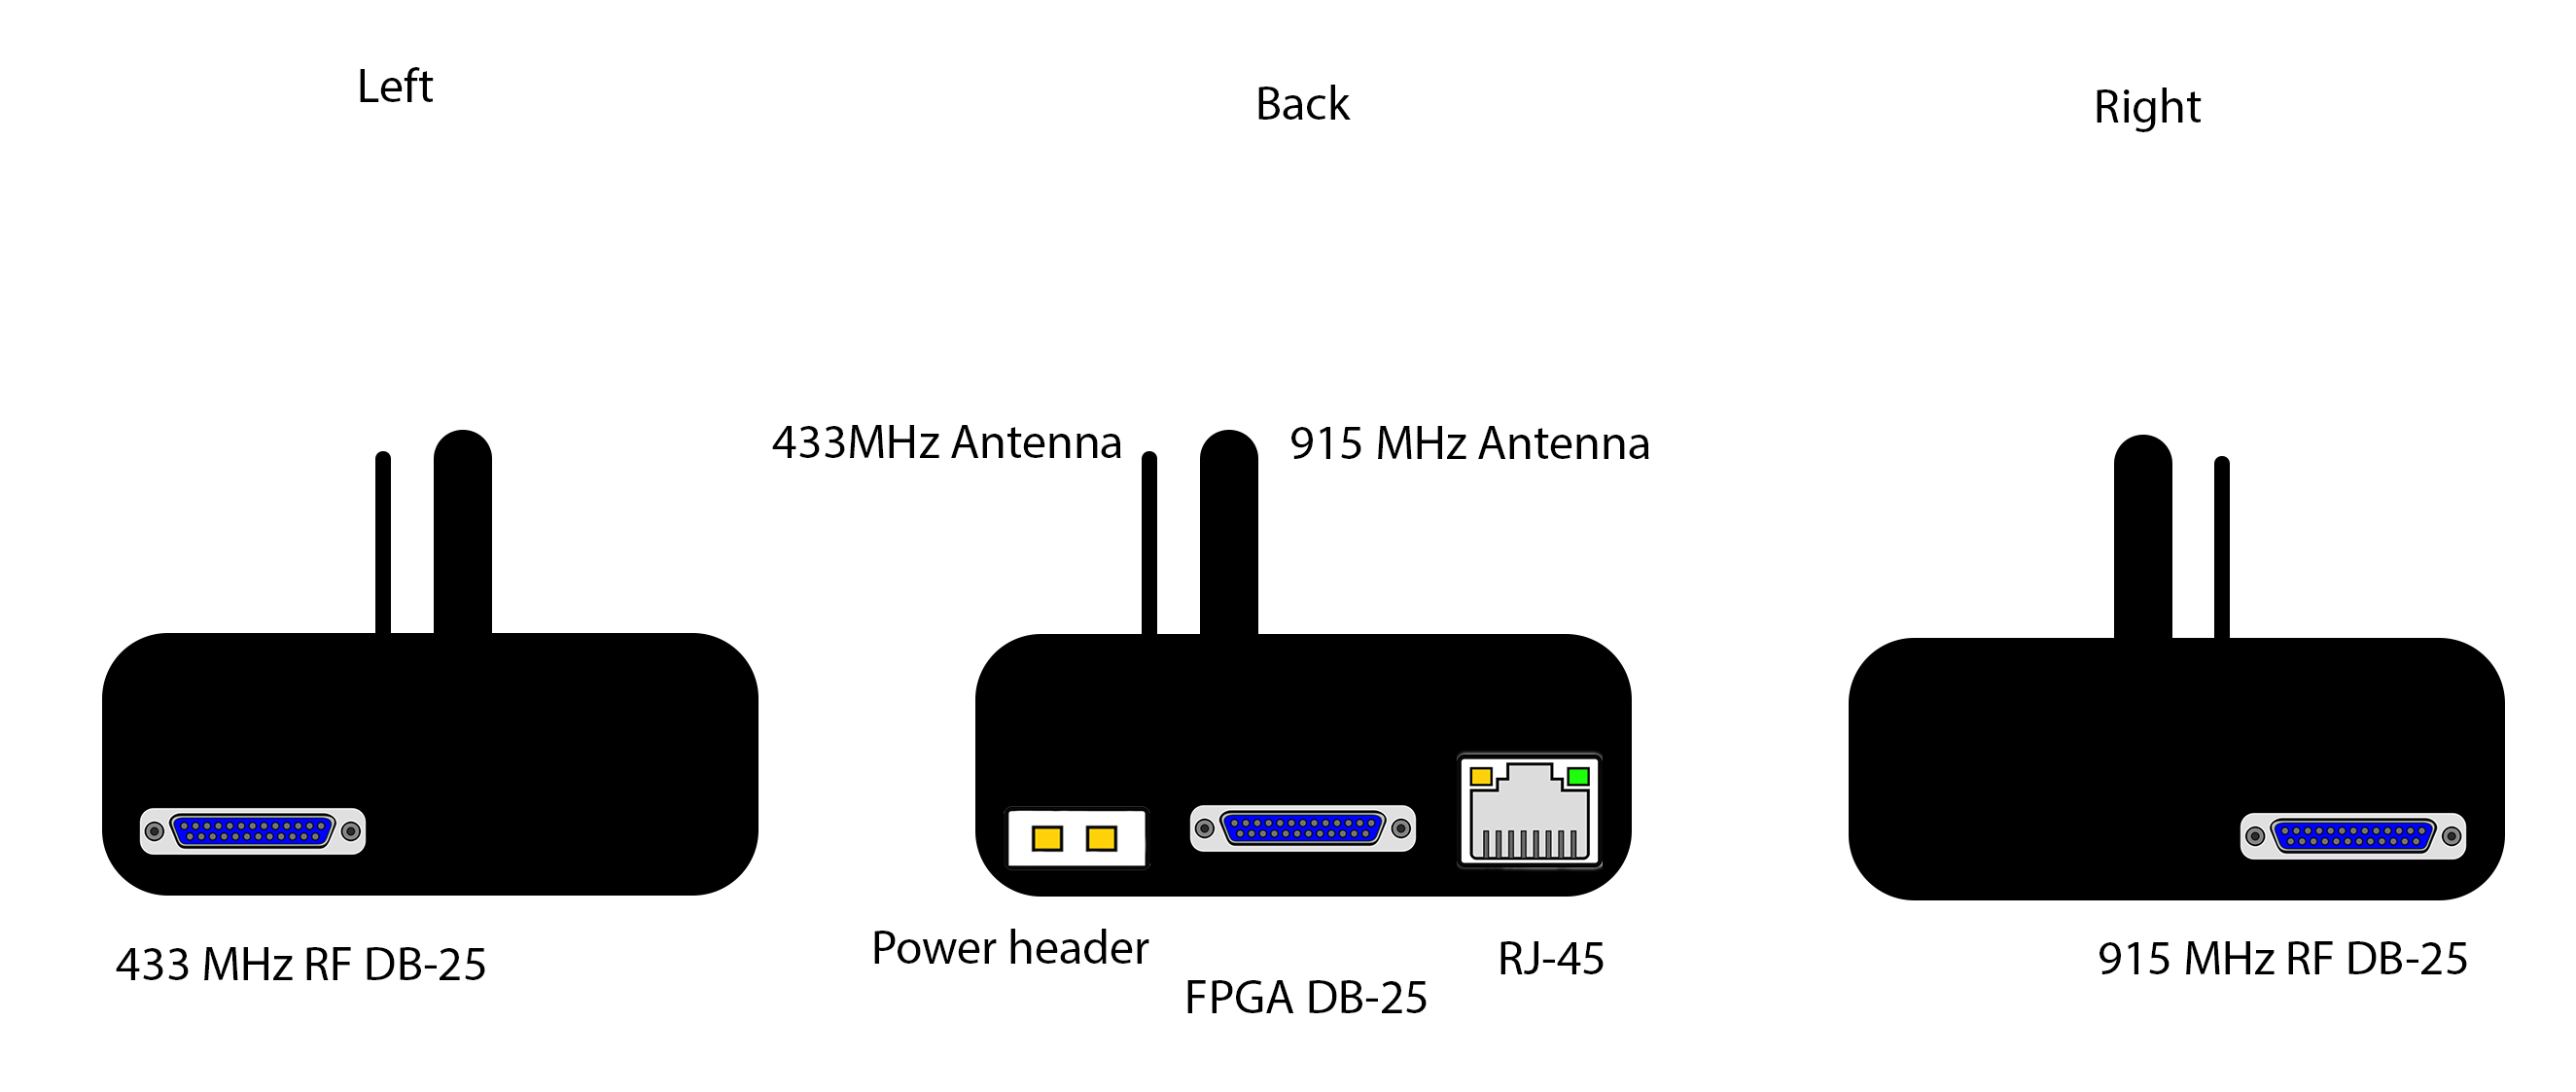
\includegraphics[width=14cm]{overview.png}
	\caption{An overview of the RF device}
	\label{fig:overview}
\end{figure}
% section device_overview (end)


\section{Configuring the Device to a Network} % (fold)
\label{sec:configuring_the_device_on_a_network}
The network interface is driven by a Lantronix xPort module. Configuring of the device can be done through the web configuration. To access the web configuration, take the following steps.
\begin{enumerate}
	\item Power the device and connect it via a CAT cable to a computer or network.
	\item Run the \texttt{getDeviceIP.sh} script.
	\item Enter the MAC address found on the device separating the pairs by colons (:). If the first character of a pair is 0, only enter the non-zero character. If both are zero, enter `0'.
	\item When prompted to open the web configuration, type ``Y''.
	\item Leave the username and password credentials blank and press ``Log In''.
	\item You will now be able to access the device settings. Select ``Network'' from the left menu to configure IP settings. The page will look as shown in Figure~\ref{fig:xnet}.
	\begin{figure}[tbh!]
		\centering
		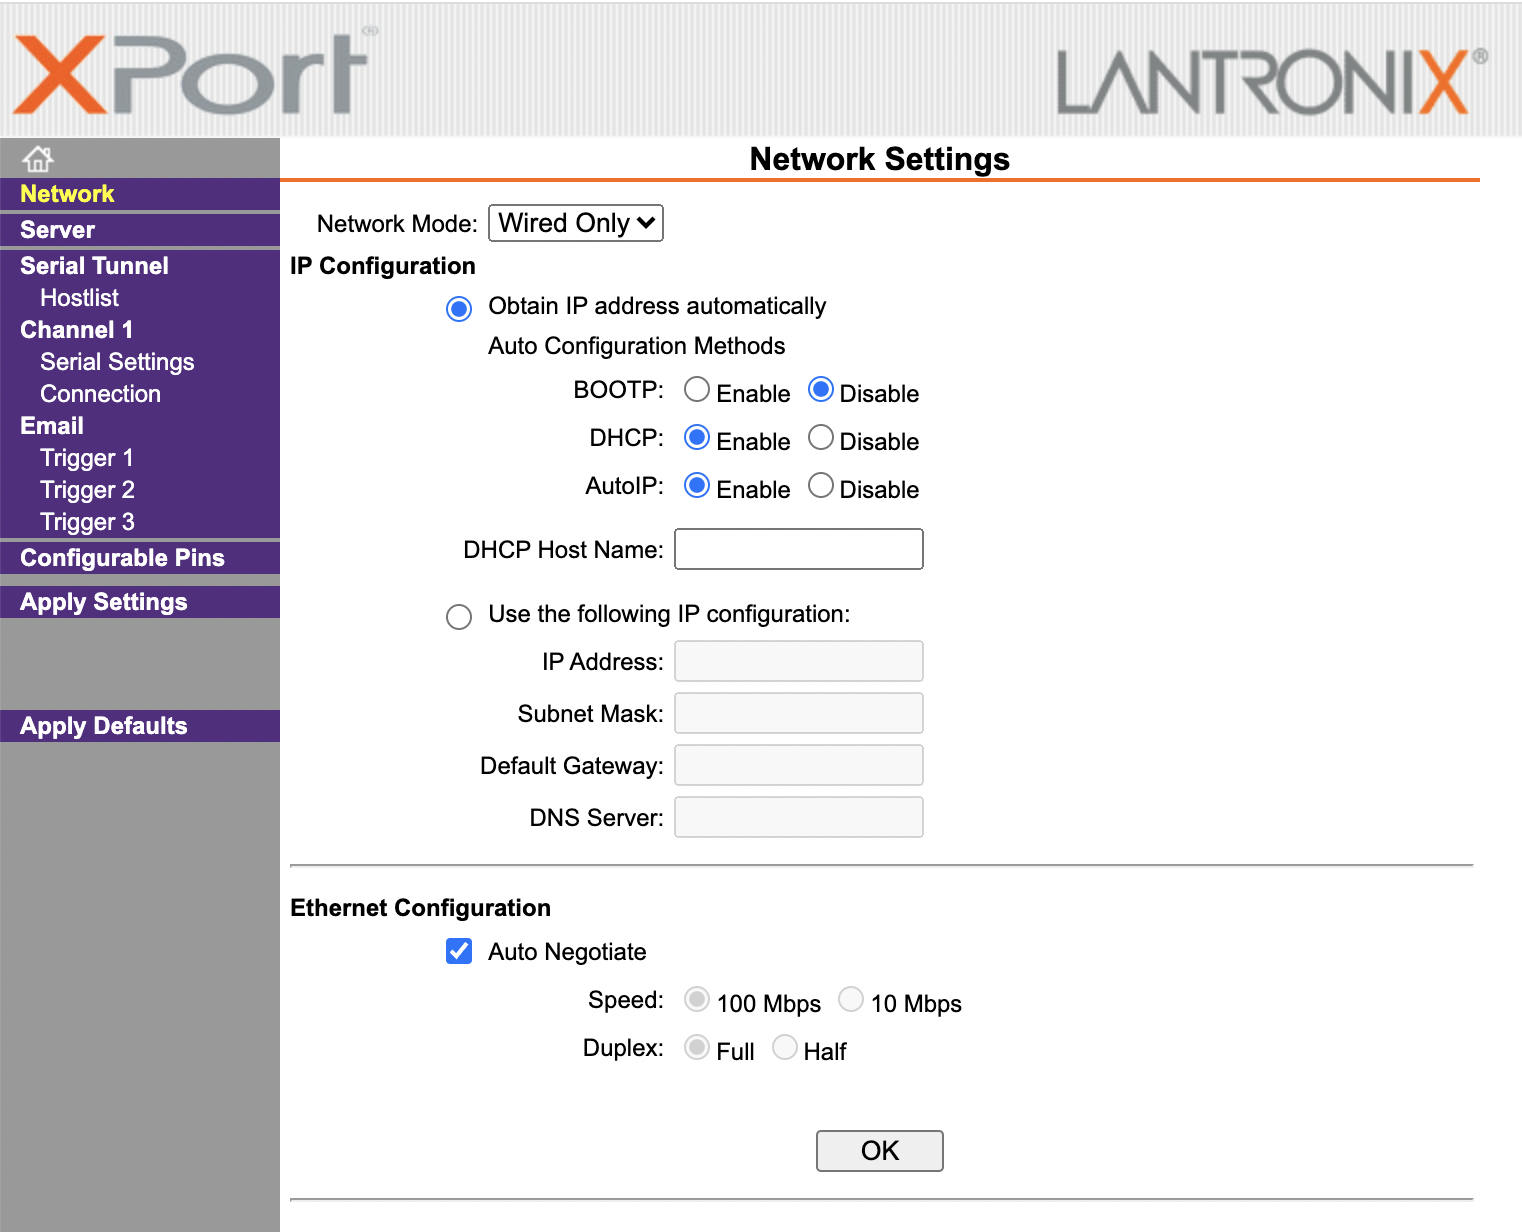
\includegraphics[width=8cm]{xPortNetwork.png}
		\caption{Network settings of the Device}
		\label{fig:xnet}
	\end{figure}
	\item In order to configure a static IP address on the device, select the ``Use the following IP configuration'' radio button.
	\item Type the desired IP, Subnet mask in the text boxes below. It is advised to leave the Default Gateway and DNS Server blank.
	\item Click the ``OK'' button at the bottom of the screen, and then the ``Apply Settings'' button in the left menu. The system will reboot with the newly assigned IP address.
\end{enumerate}

\subsection{Identification Troubleshooting} % (fold)
\label{sub:identification_troubleshooting}
If the \texttt{getDeviceIP.sh} script fails, please try the following troubleshooting methods.
\begin{enumerate}
	\item Ensure the device is powered on and green status LED is lit.
	\item If the device was connected directly to a computer, the computer IP address address may need to be changed to the following static IP format:
	\begin{description}
		\item[IP] \texttt{169.254.X.X}
		\item[Subnet Mask] \texttt{255.255.0.0}  
	\end{description}
	Where an `X' can be any number between 1-254.
	When the devices auto IP is enabled and it is connected directly to a computer it may take some time for a self assigned IP to resolve and show on the network.
	\item Check your devices firewall settings.
\end{enumerate}
% section troubleshooting_network (end)

Full instructions on configuration of the xPort module and further troubleshooting can be found at \href{https://www.lantronix.com/products/xport/}{the Lantronix Website}. Please note changing of settings not mentioned in this manual may cause unexpected behaviour of the device.
% subsection identification_troubleshooting (end)


\section{Configuring Other Network Interface Options} % (fold)
\label{sec:configuring_other_network_interface_options}
This design uses TCP protocol to communicate with other devices. UDP protocol can be used at the users own risk and configuration instructions can be found at \href{https://www.lantronix.com/products/xport/}{the Lantronix Website}.
\subsection{Changing the TCP Port} % (fold)
\label{sub:changing_the_tcp_port}
To change the TCP port take the following steps
\begin{enumerate}
	\item Follow steps 1 to 5 in Section~\ref{sec:configuring_the_device_on_a_network} to open the network configuration options.
	\item Select ``Connection'' under ``Channel 1'' in the left menu.
	\item Find the ``Port'' option and change to the number of your choice.
	\item Click the ``OK'' button at the bottom of the screen, and then the ``Apply Settings'' button in the left menu. The system will reboot with the new settings.
\end{enumerate}
% subsection changing_the_tcp_port (end)
% section configuring_other_network_interface_options (end)

\section{Configuring the FPGA Through JTAG} % (fold)
\label{sec:configuring_the_fpga_through_jtag}
To flash the FPGA configuration permanently to the module the following steps should be taken.
\begin{enumerate}
	\item Power the device and connect  the  DB-25 end of the DB-25 cable to the FPGA DB-25 connector on the device (see Figure~\ref{fig:overview}) and the other end to the computer.
	\item Follow the instructions to download and install Quartus Prime Lite \href{https://fpgasoftware.intel.com/}{here}
	\item Run the Quartus Programmer software. You will be presented with the screen shown in Figure~\ref{fig:ProgBlank}.
	\begin{figure}[tbh!]
		\centering
		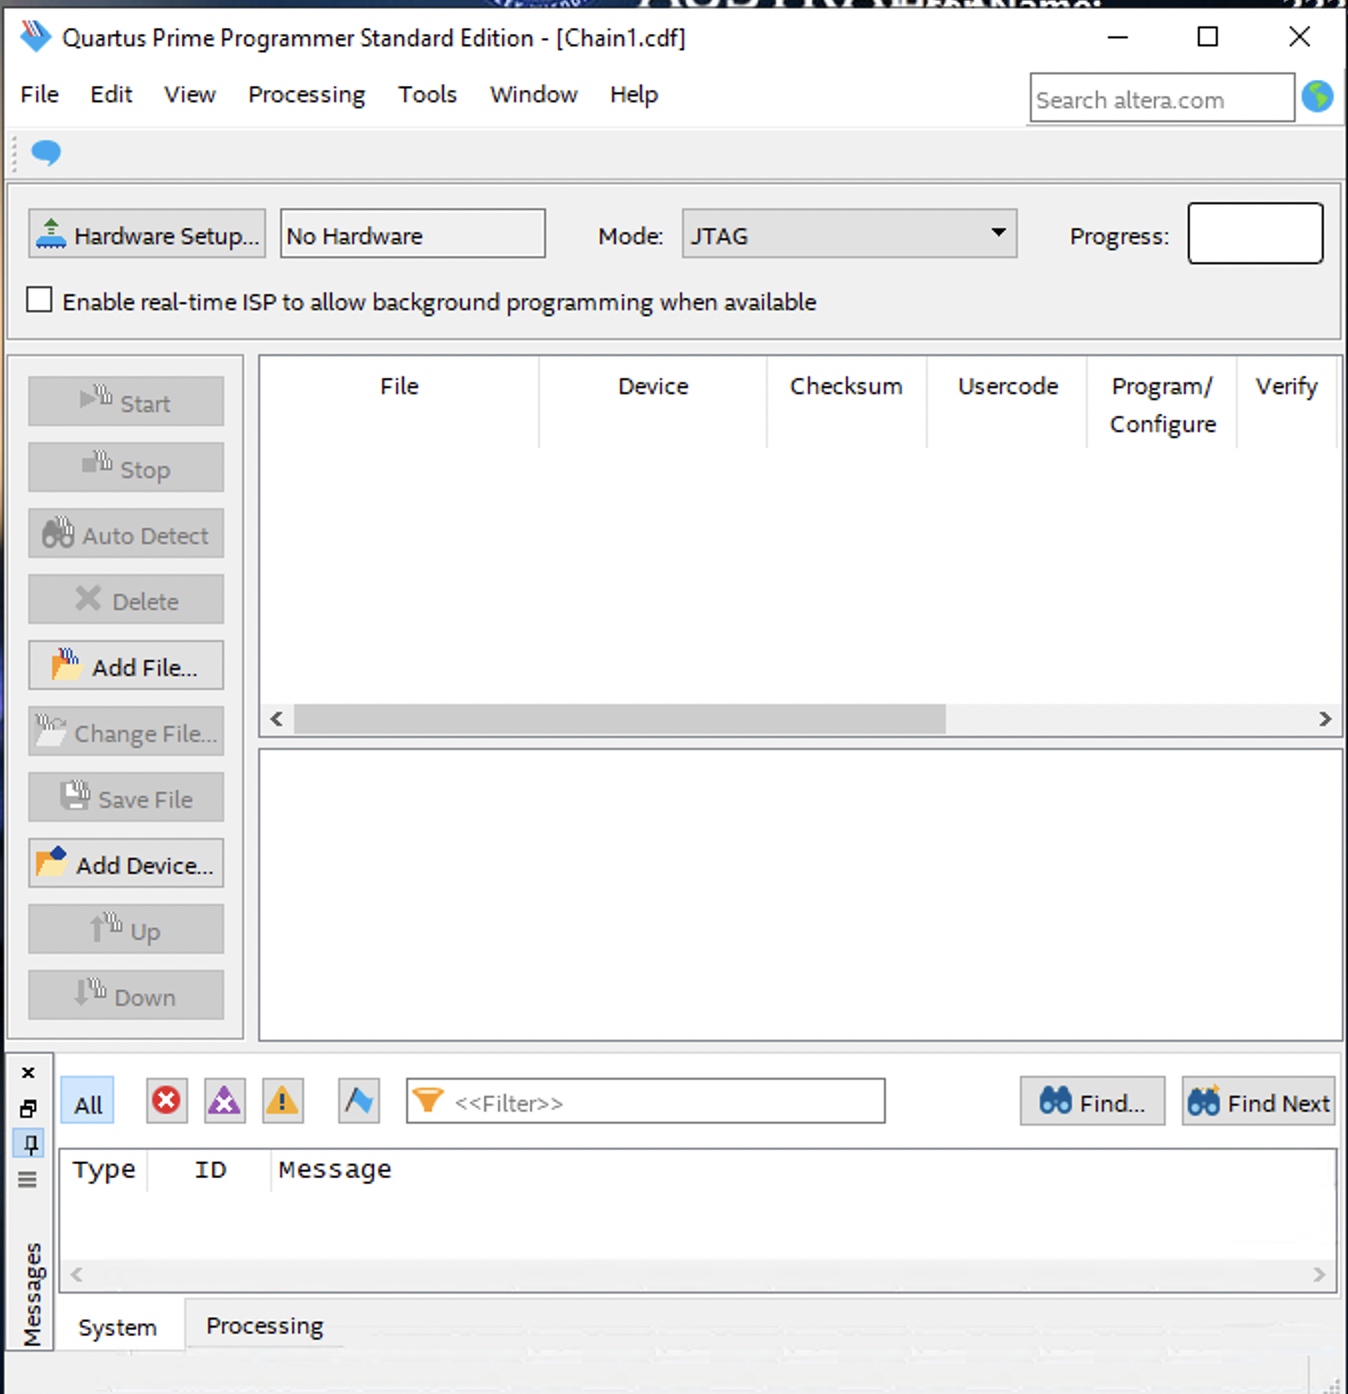
\includegraphics[width=8cm]{programmerBlank.png}
		\caption{Programmer Interface Upon Launching}
		\label{fig:ProgBlank}
	\end{figure}
	\item Click the ``Add File...'' button on the left menu and navigate to the \texttt{.pof} file and click ``Open''.
	\item Tick the checkbox under the ``Program/Configure'' heading in the table.
	\item Click ``Hardware Setup'' in the top left corner and select the available device.
	\item Ensure the mode is set to ``JTAG''.
	\item Click the ``Start'' button on the left and wait until the progress bar in the top right reaches 100 and reads ``Success''.
	\item Disconnect the DB-25 connector.
\end{enumerate}
% section configuring_the_fpga_through_jtag (end)
\section{Configuring the CC1310} % (fold)
\label{sec:configuring_the_cc1310}
To flash the CC1310 configuration to the chip:
\begin{enumerate}
	\item Follow the instructions to download and install Code Composer Studio \href{https://www.ti.com/tool/CCSTUDIO/}{here}.
	\item Import the transmit or receive CC1310 project files into CCS as shown in Figure~\ref{fig:CCSimport}.
	\begin{figure}[tbh!]
		\centering
		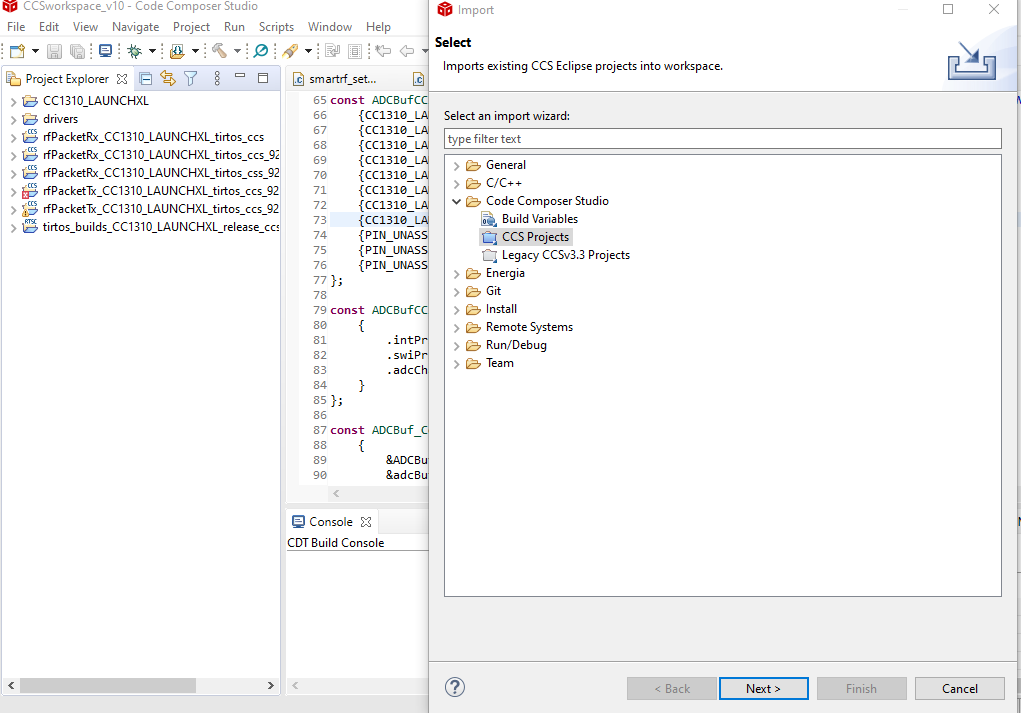
\includegraphics[width = 8cm]{import.png}
		\caption{Importing the Project Files}
		\label{fig:CCSimport}
	\end{figure}
	\item Build or rebuild project to compile as shown in Figure~\ref{fig:CCSBuild}.
	\begin{figure}[tbh!]
		\centering
		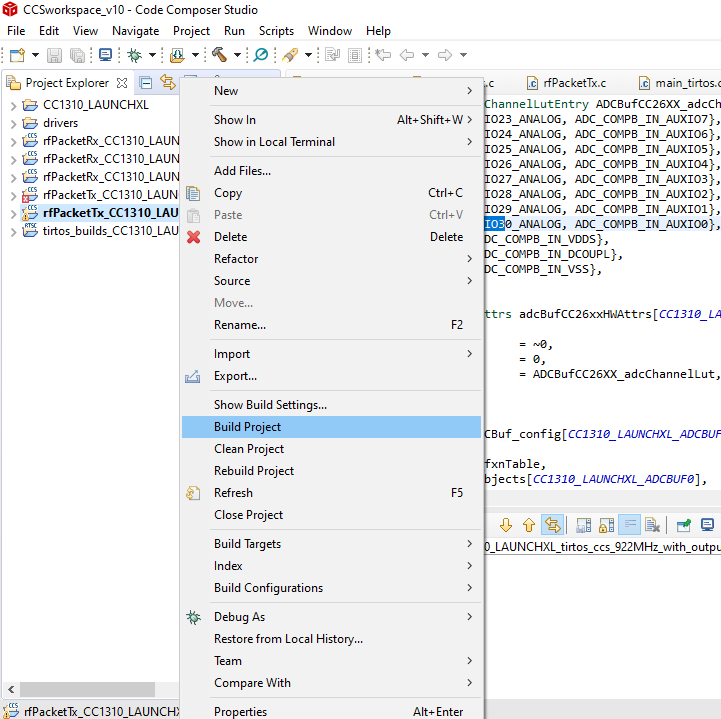
\includegraphics[width=8cm]{build.png}
		\caption{Building Project}
		\label{fig:CCSBuild}
	\end{figure}
	\item If the build is successful a notification such as the one shown in Figure~\ref{fig:CCSSuccess} will be displayed.
	\begin{figure}[tbh!]
		\centering
		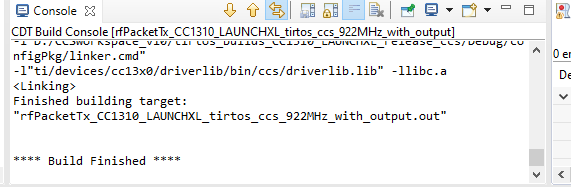
\includegraphics[width=8cm]{success.png}
		\caption{Successful build notification}
		\label{fig:CCSSuccess}
	\end{figure}
	\item Finally, start debug session to flash the program into CC1310 as in Figure~\ref{fig:CCSDebug}.
	\begin{figure}[tbh!]
		\centering
		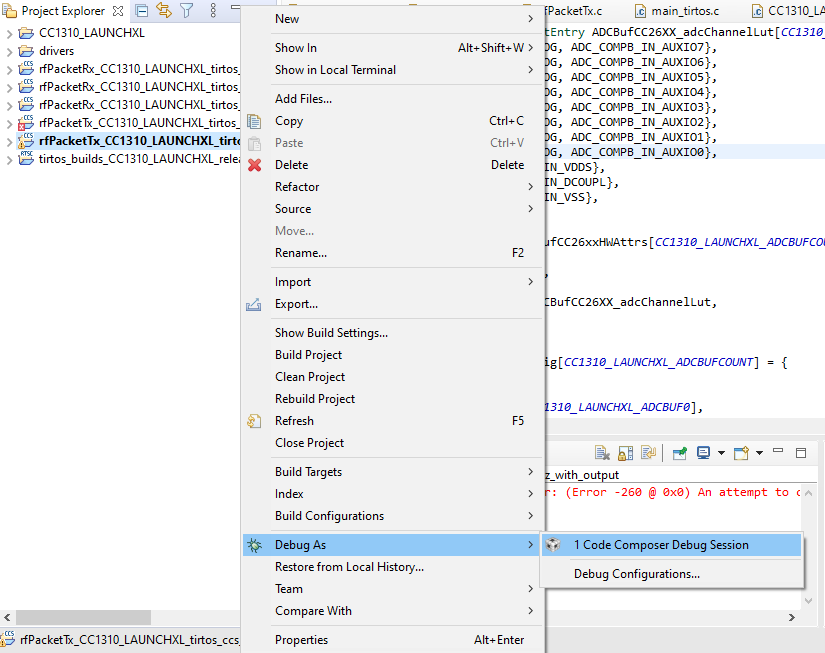
\includegraphics[width = 8cm]{debug.png}
		\caption{Begin debugging session}
		\label{fig:CCSDebug}
	\end{figure}
\end{enumerate}

These steps will need to be repeated for the transmitter and the receiver. The device utilises two distinct radio frequency bands, in the \SI{433}{\mega\hertz} range and the \SI{915}{\mega\hertz} range. The design team suggests the following configuration in Table~\ref{tab:RFconfig}. Ports to load these configs are found in Figure~\ref{fig:overview}

\begin{table}[tbh!]
	\caption{Suggested RF configuration}
	\label{tab:RFconfig}
	\centering

	\begin{tabular}{|l|c|c|}
	\hline
	\textbf{} & \textbf{Server Device} & \textbf{Remote Device} \\
	\hline
		\textbf{\SI{433}{\mega\hertz}} & Transmit & Receive\\
	\hline
		\textbf{\SI{915}{\mega\hertz}} & Receive & Transmit \\
	\hline
	\end{tabular}
\end{table}



% section configuring_the_cc1310 (end)

\section{Installing the Device} % (fold)
\label{sec:installing_the_device}
\subsection{Installing the Remote Device} % (fold)
\label{sub:installing_the_remote_device}
\subsubsection{Powering the device} % (fold)
\label{ssub:powering_the_device}
In order to power the device, connect a \SIrange{10}{36}{\volt} DC power supply available from the equipment to the power and ground headers on the device PCB.
% subsubsection powering_the_device (end)
\subsubsection{Connecting the device to equipment} % (fold)
\label{ssub:connecting_the_device_to_equipment}
Connection to the equipment can be made using a CAT cable connecting one end to the RJ-45 port on the device and the other to the RJ-45 port on the equipment.
% subsubsection connecting_the_device_to_equipment (end)
\subsubsection{Securing the device on the equipment} % (fold)
\label{ssub:securing_the_device_on_the_equimpent}
Mounting the device will depend on the nature of equipment. Please consider the following when finding a mounting point on mobile equipment.
\begin{itemize}
	\item Do not mount the device on a surface which may rotate or extend beyond the length of the attached cables as this may cause damage to the device or equipment.
	\item Do not mount the device in an area which may be exposed to impacts.
	\item Do not mount the device in a metal enclosure as this may reduce the communication range of the device.
\end{itemize}
% subsubsection securing_the_device_on_the_equimpent (end)
% subsection installing_the_remote_device (end)
\subsection{Installing the Static Device} % (fold)
\label{sub:installing_the_static_device}
\label{ssub:powering_the_device}
In order to power the device, connect a \SIrange{10}{36}{\volt} AC/DC power converter to the power and ground headers on the device PCB and connect to the mains power.
% subsubsection powering_the_device (end)
\subsubsection{Connecting the device to equipment} % (fold)
\label{ssub:connecting_the_device_to_equipment}
Connection to the network can be made using a CAT cable connecting one end to the RJ-45 port on the device and the other to a network switch or computer.
% subsection installing_the_static_device (end)
% section installing_the_device (end)


\section{Troubleshooting} % (fold)
\label{sec:troubleshooting}
The device is equipped with a reset button which will reset all the sub-systems of the device. If prior troubleshooting methods have been tried use this reset button to reset the device.
% section troubleshooting (end)

\section{Conclusion} % (fold)
\label{sec:conclusion}
After following the above steps, the device will be fully configured. TCP connections can be established on both the mobile equipment and server side to pass data between the two devices over wireless radio transmission.
% section conclusion (end)